\chapter{Week5}
\section{Monday for MAT3040}\index{Monday_lecture}
\paragraph{Reviewing}
\begin{itemize}
\item
Dual space: the set of linear transformations from $V$ to $\mathbb{F}$, denoted as $\text{Hom}(V,\mathbb{F})$.
\item
Suppose $B=\{\bm v_i\mid i\in I\}$ is the basis of $V$, define $B^*=\{f_i\mid i\in I\}$ by
\[
f_i(\bm v_j) = \delta_{ij}=\left\{
\begin{aligned}
1,&\quad i=j\\
0,&\quad i\ne j
\end{aligned}
\right.
\]
Actually, the above recipe uniquely defines a linear transformation $f_i:V\to\mathbb{F}$: For any $\bm v\in V$, it can be written as $\bm v = \sum_{i\in I}\alpha_i\bm v_i$, and therefore
\[
f_i(\bm v)=f_i(\sum_{i\in I}\alpha_i\bm v_i)= \sum_{i\in I}\alpha_if_i(\bm v_i).
\]

\begin{example}
Consider $V=\mathbb{R}^n, B=\{\bm e_1,\dots,\bm e_n\}$. Then we imply $B^*=\{\phi_i\}_{i=1}^n$, where $\phi_i$ is the mapping $V\to\mathbb{R}$ defined by
\[
\phi_i\begin{pmatrix}
x_1\\\vdots\\ x_n
\end{pmatrix}=\phi(x_1\bm e_1+\cdots+x_n\bm e_n)=\sum_{j=1}^nx_j\phi_i(\bm e_j) = x_i
\]
\end{example}
\end{itemize}


\subsection{Remarks on Dual Space}
\begin{proposition}\label{pro:5:1}
\begin{enumerate}
\item
$B^*$ is always lienarly independent, i.e., any finite subset of $B^*$ is linearly independent.
\item
If $V$ has finite dimension, then $B^*$ is a basis of $V^*$.
\end{enumerate}

\end{proposition}
\begin{proof}
\begin{enumerate}
\item
Suppose that 
\[
\alpha_1 f_{i_1}+\alpha_2 f_{i_2}+\cdots+\alpha_k f_{i_k} = \bm0_{V^*}.
\]
In particular, let the input of these linear transformations be $\bm v_{i_1}$, we imply
\begin{align*}
\alpha_1 f_{i_1}(\bm v_{i_1})+\alpha_2 f_{i_2}(\bm v_{i_1})+\cdots+\alpha_k f_{i_k}(\bm v_{i_1}) &= \bm0(\bm v_{i_1})\equiv\bm0\\
&=\alpha_1\cdot1+\cdots+0\\
&=\alpha_1
\end{align*}
Applying the same trick, one can show that $\alpha_2=\cdots=\alpha_k=0$. 
Therefore, $\{f_{i_1},\dots,f_{i_k}\}$ is linearly independent.
\item
Suppose that $B=\{\bm v_1,\dots,\bm v_n\}$ and $B^*=\{f_1,\dots,f_n\}$.
For any $f\in V^*$, construct the linear transformation
\[
g:=\sum_{i=1}^nf(\bm v_i)\cdot f_i\in\Span\{B^*\}.
\]
It follows that for $j=1,2,\dots,n$,
\[
g(\bm v_j) = \sum_{i=1}^nf(\bm v_i)\cdot f_i(\bm v_j) = f(\bm v_j).
\]
It's clear that $g(\bm v) = f(\bm v)$ for all $\bm v\in V$, i.e., $f\equiv g\in\Span(B^*)$.
Therefore $B^*$ spans $V^*$, i.e., forms a basis of $V^*$.
\end{enumerate}
\end{proof}

\begin{corollary}
If $\dim(V)=n$, then $\dim(V^*)=n$.
\end{corollary}
\begin{proof}
It's eay to show the mapping defined as
\[
\begin{array}{ll}
&V\to V^*\\
\text{with }&\bm v_i\mapsto f_i
\end{array}
\]
is an isomorphism from $V\to V^*$.
Note that this constructed isomorphism depends on \emph{the choice of basis} $B$ in $V$. (We say this is not a \emph{natural isomorphism}.)
\end{proof}

\begin{remark}
The part 2 for proposition~(\ref{pro:5:1}) does not hold for $V$ with infinite dimension. The reason is that the spanning set is defined with \emph{finite} linear combinations. Check the example below for a counter-example.
\end{remark}



\begin{example}
Suppose that $V=\mathbb{F}[x]$, and $B^* = \{1,x,x^2,\dots,\}$ forms a basis of $V$. 
We imply that $B^*=\{\phi_0,\phi_1,\phi_2,\dots,\}$, where $\phi_i$ is the mapping defined as
\[
\phi_i(x^j) = \left\{
\begin{aligned}
1,&\quad i=j\\
0,&\quad\text{otherwise}
\end{aligned}
\right.
\]
Consider a special element $\phi\in V^*$ with $f(p(x)) = p(1)$:
\[
\begin{array}{lllll}
\phi(1)=1,&\phi(x)=1,&\phi(x^2)=1,&\cdots&\phi(x^n)=1,\quad\forall n\in\mathbb{N}.
\end{array}
\]
If following the proof in proposition~(\ref{pro:5:1}), we expect that 
\[
g := \sum_{n=0}^\infty \phi(x^n)\phi_n = \sum_{n=0}^\infty \phi_n\in\Span\{B^*\},
\]
which is a contradiction, since $\Span\{B^*\}$ consists of finite sum of $\phi_i$'s only.
\end{example}
\begin{remark}
Therefore, if $V$ is not finite-dimensional, we can say the cardinality of $V$ is strictly less than the cardinality of $V^*$.
\end{remark}

Any subspace of a given vector space has some gap. Now we want to describe this gap formally from the perspective of the dual space.

\subsection{Annihilators}
\begin{definition}
Let $V$ be a vector space, $S\subseteq V$ be a subset.
The \emph{annihilator} of $S$ is defined as
\[
\text{Ann}(S) = \{f\in V^*\mid f(s) = 0,\forall s\in S\}
\]
\end{definition}
\begin{example}
Consider $V=\mathbb{R}^4$, $B=\{\bm e_1,\dots,\bm e_4\}$. 
Let $B^*=\{f_1,\dots,f_4\}$, $S=\{\bm e_3,\bm e_4\}$. 
\begin{itemize}
\item
Then $f_1\in\text{Ann}(S)$, since
\[
\begin{array}{ll}
f_1(\bm e_3) = 0,
&
f_1(\bm e_4)=0
\end{array}
\]
\end{itemize}
Indeed, any $a\cdot f_1+b\cdot f_2\in V^*$ is in $\text{Ann}(S)$.
\end{example}

\begin{proposition}
\begin{enumerate}
\item
The set $\text{Ann}(S)$ is a vector subspace of $V^*$
\item
The mapping $\text{Ann}(\cdot)$ is \emph{inclusion-reversing}, i.e., if $W_1\subseteq W_2\subseteq V$, then
\[
\text{Ann}(W_1)\supseteq\text{Ann}(W_2)
\] 
\item
The mapping $\text{Ann}(\cdot)$ is \emph{idempotent}, i.e.,
$\text{Ann}(S) = \text{Ann}(\Span(S))$.
\item
If $V$ has finite dimension, and $W\le V$, then $\text{Ann}(W)$ fills in the gap, i.e., 
\[
\dim(W) + \dim(\text{Ann}(W)) = \dim(V)
\]
\end{enumerate}
\end{proposition}
\begin{proof}
\begin{enumerate}
\item
Suppose that $f,g\in\text{Ann}(S)$, i.e., $f(s) = g(s)=0,\forall s\in S$. 
It's clear that $(af+bg)\in\text{Ann}(S)$.
\item
Suppose that $f\in\text{Ann}(W_2)$, we imply $f(\bm w)=0$ for any $\bm w\in W_2$.
Therefore, $f(\bm w_1)=0$ for any $\bm w_1\in W_1\subseteq W_2$, i.e., $f\in\text{Ann}(W_1)$.
\item
Note that $S\subseteq\Span(S)$. Therefore we imply $\text{Ann}(S)\supseteq\text{Ann}(\Span(S))$ from part $(b)$.
It suffices to show $\text{Ann}(S)\subseteq\text{Ann}(\Span(S))$:

For any $f\in \text{Ann}(S)$ and any $\sum_{i=1}^nk_i\bm s_i\in\Span(S)$, we imply
\begin{align*}
f\left(\sum_{i=1}^nk_i\bm s_i\right)&=\sum_{i=1}^nk_if(\bm s_i)\\
&=\sum_{i=1}^nk_i\cdot 0\\
&=0,
\end{align*}
i.e., $f\in\text{Ann}(\Span(S))$.
\item
Let $\{\bm v_1,\dots,\bm v_k\}$ be a basis of $W$.
By basis extension, we construct a basis of $V$:
\[B=\{\bm v_1,\dots,\bm v_k,\bm v_{k+1},\dots,\bm v_n\}.\] 

Let $B^*=\{f_1,\dots,f_k,f_{k+1},\dots,f_n\}$ be a basis of $V^*$. 
We claim that $\{f_{k+1},\dots,f_n\}$ is a basis of $\text{Ann}(W)$:

\begin{itemize}
\item
Firstly, $f_j$'s are the elements in $\text{Ann}(W)$ for $j=k+1,\dots,n$, since for any $\bm w=\sum_{i=1}^k\alpha_i(\bm v_i)\in W$, we have
\begin{align*}
f_{j}(\bm w)&=\sum_{i=1}^k\alpha_if_j(\bm v_i)\\
&=\sum_{i=1}^k\alpha_i\cdot0\\
&=0,\quad j=k+1,k+2,\dots,n
\end{align*}
\item
Secondly, the set $\{f_{k+1},\dots,f_n\}$ is linearly independent, since the set $B^*=\{f_{1},\dots,f_n\}$ is linearly independent.
\item
Thirdly, $\{f_{k+1},\dots,f_n\}$ spans $\text{Ann}(W)$: for any $g\in\text{Ann}(W)\subseteq V^*$, it can be expressed as $g=\sum_{i=1}^n\beta_if_i$. It follows that
\begin{align*}
g(\bm v_1)&=\sum_{i=1}^n\beta_if_i(\bm v_1)=0\implies\beta_1=0\\
\vdots\\
g(\bm v_k)&=\sum_{i=1}^n\beta_if_i(\bm v_k)=0\implies\beta_k=0\\
\end{align*}
Substituting $\beta_1=\cdots=\beta_k=0$ into $g=\sum_{i=1}^n\beta_if_i$, we imply 
\[
g = \beta_{k+1}f_{k+1}+\cdots+\beta_nf_n\in\Span\{f_{k+1},\dots,f_n\}.
\]
\end{itemize}
Therefore, $\{f_{k+1},\dots,f_n\}$ forms a basis for $\text{Ann}(W)$, i.e., $\dim(\text{Ann}(W)) = n-k$.
\end{enumerate}
\end{proof}

\begin{remark}
Let $W\le V$, where $V$ has finite dimension, recall that we have obtained two relations below:
\begin{align*}
\dim(\text{Ann}(W)) &= \dim(V) - \dim (W)\\
\dim((V/W)^*)&=\dim(V/W)=\dim(V) - \dim(W)
\end{align*}
Therefore, $\dim((V/W)^*)=\dim(\text{Ann}(W))$, i.e., 
\[
(V/W)^*\cong\text{Ann}(W).
\]
The question is that can we construct an isomorphism explicitly?
We claim that the mapping defined below is an isomorphism:
\[
\begin{array}{ll}
&\text{Ann}(W)\to(V/W)^*\\
\text{with }&f\mapsto \tilde{f},
\end{array}
\]
where $\tilde f:V/W\to\mathbb{F}$ is constructed from the \emph{universal property I}, i.e., given the mapping $f\in\text{Ann}(W)$, since $W\le\ker(f)$, there exists $\tilde f:V/W\to\mathbb{F}$ such that the diagram below commutes:
\begin{figure}[H]
\centering
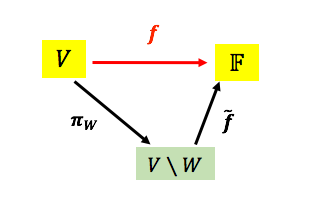
\includegraphics[width=0.6\textwidth]{week5/p_1}
\end{figure}
i.e., $\tilde{f}(\bm v+W)=f(\bm v)$.
\end{remark}























